\documentclass[11pt,a4paper]{article}

% --- Fonts & Encoding ---
\usepackage[T1]{fontenc}
\usepackage[utf8]{inputenc}
\usepackage{newtxtext,newtxmath}
\usepackage[english]{babel}

% --- Page Layout ---
\usepackage[margin=1in,includefoot]{geometry}

% --- Graphics & Figures ---
\usepackage{graphicx}
\usepackage{subcaption}
\usepackage{float}

% --- Math ---
\usepackage{amsmath,amsthm}
\usepackage{bm}
\usepackage{mathtools}

% --- Tables ---
\usepackage{booktabs}
\usepackage{multirow}
\usepackage{array}

% --- Code Listings ---
\usepackage{listings}
\usepackage{xcolor}

\lstset{
  basicstyle=\ttfamily\small,
  breaklines=true,
  frame=single,
  numbers=left,
  numberstyle=\tiny\color{gray},
  keywordstyle=\color{blue}\bfseries,
  commentstyle=\color{gray}\itshape,
  stringstyle=\color{red},
  tabsize=2,
  captionpos=b
}

% --- Hyperlinks ---
\usepackage[hidelinks]{hyperref}
\usepackage{url}

% --- Bibliography ---
\usepackage[numbers,sort&compress]{natbib}

% --- Theorem environments ---
\newtheorem{theorem}{Theorem}[section]
\newtheorem{corollary}{Corollary}[theorem]
\newtheorem{lemma}[theorem]{Lemma}
\theoremstyle{definition}
\newtheorem{definition}{Definition}[section]

% --- Operators ---
\DeclareMathOperator{\Softmax}{softmax}
\DeclareMathOperator{\LayerNorm}{LayerNorm}
\DeclareMathOperator{\SelfAttn}{SelfAttn}
\DeclareMathOperator{\CrossAttn}{CrossAttn}
\DeclareMathOperator{\FFN}{FFN}
\DeclareMathOperator{\Embed}{Embed}

% --- Title ---
\title{Applying the Brain's Dual-Library Mechanism\\to Transformer Architectures}
\author{Heiko Wagner\\
  \small Independent Researcher, Bonn, Germany\\
  \small \texttt{heikowagner@t-online.de}
}
\date{June 2026}

\begin{document}
\maketitle

\begin{abstract}
Current large language models (LLMs) concatenate system instructions, historical context, and factual data into the same token sequence. Through successive layers of self-attention, these distinct inputs intertwine—a monolithic blending that creates structural vulnerabilities: context drift, prompt injection, and the ``lost in the middle'' phenomenon. A landmark single-neuron recording study by Bausch et al.\ (2026) \cite{bausch2026distinct} suggests a biological alternative: human memory maintains a functional separation between \emph{what} occurs (content) and the framework within which it occurs (context). This paper proposes a dual-stream Transformer that mirrors this separation. Isolated content and context streams, coupled through unidirectional cross-attention with a content-driven sigmoidal gate, yield three concrete benefits: mathematically guaranteed prompt injection resistance (proved by induction over transformer layers), mitigation of lost-in-the-middle degradation, and improved zero-shot generalisation through context-invariant representations. In a controlled experiment with 1,750 samples across 10 task categories, the dual-stream Transformer achieves a 1.69$\times$ improvement in validation loss over a parameter-matched monolithic baseline, with a substantially smaller generalisation gap.
\end{abstract}

% ============================================================================
\section{Introduction}
% ============================================================================

Transformer-based large language models \cite{Vaswani2017AttentionIA} process all input tokens through a unified self-attention mechanism. System instructions, conversation history, and factual data are concatenated into a single sequence—through successive layers, tokens representing entirely different semantic functions freely attend to one another. This design, while remarkably effective for next-token prediction, introduces structural vulnerabilities that scale with context length.

Three problems are well documented. First, \textbf{prompt injection}: an adversarial user input can override system instructions because all tokens share the same attention space~\cite{promptinjection2022}. Current defences rely on training data quality and reinforcement learning from human feedback (RLHF), both of which are inherently adversarial—a determined attacker can always find prompts outside the training distribution. Second, the \textbf{``lost in the middle''} phenomenon~\cite{lostinthemiddle2023}: as context windows grow to millions of tokens, models increasingly overlook information placed in the centre of the input because attention weights dilute across an undifferentiated token pool. Third, \textbf{context drift}: long context windows degrade the precision of content representations because contextual tokens mask factual tokens.

A recent single-neuron recording study from the University of Bonn~\cite{bausch2026distinct} suggests a radically different approach. Bausch et al.\ recorded 3,109 single neurons in the human medial temporal lobe and identified two largely distinct neuronal populations: stimulus neurons (invariant to task context) and context neurons (invariant to stimulus identity). Only 1.61\% of neurons showed significant stimulus--context interaction. Crucially, the connection between the two populations is asymmetric and directional: firing of stimulus neurons in the entorhinal cortex predicted firing of context neurons in the hippocampus after approximately 40\,ms, but not the reverse.

This paper translates these findings into a concrete Transformer architecture. The contributions are:
\begin{enumerate}
  \item A \textbf{dual-stream Transformer} with separate weight matrices for content and context streams, coupled through unidirectional cross-attention with a content-driven sigmoidal gate.
  \item A \textbf{mathematical proof} by induction over transformer layers that the content stream has no computational path into the context stream ($\partial H_{\text{ctx}} / \partial x_c = 0$), establishing a structural guarantee against prompt injection.
  \item An \textbf{experimental validation} on a 1,750-sample corpus across 10 task categories, showing 1.69$\times$ better validation loss and substantially reduced overfitting compared to a parameter-matched monolithic baseline.
\end{enumerate}

% ============================================================================
\section{Biological Paradigm}
% ============================================================================

Bausch et al.\ recorded 3,109 single neurons in the amygdala, parahippocampal cortex, entorhinal cortex, and hippocampus while patients performed a comparison task: pairs of pictures appeared on screen, and a question shown at the start of each trial specified the comparison rule—\emph{``Which is bigger?''}, \emph{``Which did you see more recently in real life?''}, \emph{``Which is brighter?''}. The question defined the task context; the pictures were the content.

The study identified two largely distinct neuronal populations in the medial temporal lobe:

\begin{itemize}
  \item \textbf{Stimulus neurons} (597 identified)—fire selectively to specific picture content, regardless of which question context is active. Most (88\%) are invariant to context.
  \item \textbf{Context neurons} (200 identified)—fire selectively to a particular task context (question), regardless of which picture is shown. Most (63.5\%) are invariant to stimulus identity.
\end{itemize}

Across all 3,109 neurons, only 50 (1.61\%) showed significant stimulus--context interaction—i.e., responded to specific picture--question combinations. Instead, separate orthogonal populations represent content and context independently, combining them via co-activation and reinstatement.

The critical architectural insight comes from the temporal dynamics: firing of stimulus neurons in the entorhinal cortex predicted firing of context neurons in the hippocampus after approximately 40\,ms—\textbf{but not the reverse}. Context neurons showed increased excitability after pre-activation by their preferred question—a gating mechanism where prior context exposure guides which hippocampal context representations are reinstated when a stimulus is subsequently encountered. This directional asymmetry and gating behaviour are the key properties this paper translates directly into a transformer layer.

% ============================================================================
\section{Dual-Stream Transformer Architecture}
% ============================================================================

In standard Transformer models~\cite{Vaswani2017AttentionIA}, query $Q$, key $K$, and value $V$ matrices are computed across the entire token sequence simultaneously:

\begin{equation}\label{eq:standard_attn}
  \text{Attention}(Q, K, V) = \Softmax\left(\frac{QK^T}{\sqrt{d_k}}\right)V
\end{equation}

If a prompt contains a factual statement followed by an instruction, the token embeddings for both elements modify each other in every layer. Context and content share a vector space; a long context window degrades the precision of the content representation.

We propose to give the model two separate token sequences rather than one. Instead of prepending a system prompt to the user message and hoping the model treats them differently, the architecture routes them through distinct processing paths from the embedding layer onward:

\begin{itemize}
  \item \textbf{Content stream}—user input, documents, code, factual data (analogous to stimulus neurons).
  \item \textbf{Context stream}—system instructions, persona, output constraints (analogous to context neurons).
\end{itemize}

Each stream has its own weight matrices and is never concatenated with the other.

\subsection{Gatekeeper Cross-Attention}\label{sec:gatekeeper}

To replicate the brain's ability to reconstruct a complete memory from its parts, the architecture introduces an asymmetric cross-attention layer. The processed content acts as the driver (query), while the context serves as the lookup library (key and value):

\begin{equation}\label{eq:cross_attn}
  H_{\text{cross}} = \text{Attention}(Q_{\text{content}}, K_{\text{context}}, V_{\text{context}})
\end{equation}

This design ensures that the context cannot overwrite the content; instead, the content actively retrieves the specific structural instructions needed to format or manipulate its data.

The final step requires a mathematical gate to control information flow, mimicking the 40\,ms temporal delay observed in the Bonn study. Instead of adding the cross-attention output directly to the residual stream, the model utilises a sigmoid-controlled linear unit. Let $H_{\text{content}}$ be the hidden states of the content stream. The gate activation $G$ is defined as:

\begin{equation}\label{eq:gate}
  G = \sigma(W_g \cdot H_{\text{content}} + b_g)
\end{equation}

The final integrated representation $H_{\text{final}}$ is computed via an element-wise product:

\begin{equation}\label{eq:final}
  H_{\text{final}} = \LayerNorm\!\big(H_{\text{content}} + (G \odot H_{\text{cross}})\big)
\end{equation}

Intuitively, the gate learns to answer a simple question for each hidden dimension: \emph{does this content need external context to be processed correctly?} Since $G$ is computed from the content stream itself ($W_g \cdot H_{\text{content}}$), the model conditions its reliance on context based on what the content already communicates.

\begin{itemize}
  \item \textbf{Gate open ($G \to 1$):} The content is raw, unstructured data—\emph{``The system peaked at 180\,°C during stress testing.''} These tokens carry no inherent task signal. The gate allows retrieved context (e.g., a system prompt like ``Extract metrics as JSON'') to shape the output.
  \item \textbf{Gate closed ($G \to 0$):} The content already implies the task—\emph{``What is the capital of France?''} or \emph{``SELECT * FROM users WHERE active = 1;''}. The tokens encode their own structural intent. Injecting additional context would be redundant or conflicting, so the gate suppresses it.
\end{itemize}

This conditional routing is structurally what prevents prompt injection: tokens inside the content stream that mimic instructions are evaluated strictly as content, and the gate—having learned from training that such patterns never originate in the context path—stays closed for them.

\subsection{PyTorch Reference Implementation}

The following defines a \texttt{ContentContextLayer} that implements parallel routing, cross-attention lookup, and the asymmetric gating mechanism:

\begin{lstlisting}[language=Python, caption=ContentContextLayer implementing dual-stream processing with gatekeeper cross-attention.,label=lst:layer]
import torch
import torch.nn as nn

class ContentContextLayer(nn.Module):
    def __init__(self, d_model, nhead, dim_feedforward=2048, dropout=0.1):
        super().__init__()
        # 1. Isolated Self-Attention (Separate Neural Libraries)
        self.content_self_attn = nn.MultiheadAttention(
            d_model, nhead, dropout=dropout, batch_first=True)
        self.context_self_attn = nn.MultiheadAttention(
            d_model, nhead, dropout=dropout, batch_first=True)
        self.norm1_content = nn.LayerNorm(d_model)
        self.norm1_context = nn.LayerNorm(d_model)
        # 2. Specialized Feed-Forward Networks
        self.ffn_content = nn.Sequential(
            nn.Linear(d_model, dim_feedforward), nn.GELU(),
            nn.Dropout(dropout), nn.Linear(dim_feedforward, d_model))
        self.ffn_context = nn.Sequential(
            nn.Linear(d_model, dim_feedforward), nn.GELU(),
            nn.Dropout(dropout), nn.Linear(dim_feedforward, d_model))
        self.norm2_content = nn.LayerNorm(d_model)
        self.norm2_context = nn.LayerNorm(d_model)
        # 3. Gatekeeper and Pattern Completion
        self.cross_attn = nn.MultiheadAttention(
            d_model, nhead, dropout=dropout, batch_first=True)
        self.gate_proj  = nn.Linear(d_model, d_model)
        self.norm_final = nn.LayerNorm(d_model)
        self.dropout    = nn.Dropout(dropout)

    def forward(self, content_x, context_x,
                content_causal_mask=None, content_padding_mask=None,
                context_mask=None):
        # Phase 1: Isolated processing paths
        c_attn_out, _ = self.content_self_attn(
            content_x, content_x, content_x,
            attn_mask=content_causal_mask,
            key_padding_mask=content_padding_mask)
        content_x = self.norm1_content(content_x + self.dropout(c_attn_out))
        ctx_attn_out, _ = self.context_self_attn(
            context_x, context_x, context_x,
            key_padding_mask=context_mask)
        context_x = self.norm1_context(context_x + self.dropout(ctx_attn_out))
        # Phase 2: Feed-Forward updates
        content_x = self.norm2_content(
            content_x + self.dropout(self.ffn_content(content_x)))
        context_x = self.norm2_context(
            context_x + self.dropout(self.ffn_context(context_x)))
        # Phase 3: Gatekeeper Mechanism
        retrieved_context, _ = self.cross_attn(
            query=content_x, key=context_x, value=context_x,
            key_padding_mask=context_mask)
        gate         = torch.sigmoid(self.gate_proj(content_x))
        gated_context = gate * retrieved_context
        final_output = self.norm_final(
            content_x + self.dropout(gated_context))
        return final_output, content_x, context_x
\end{lstlisting}

% ============================================================================
\section{Training}\label{sec:training}
% ============================================================================

Training this architecture differs from standard transformer pre-training, which uses unstructured text streams where the boundary between instructions and data is undefined. The network requires paired inputs at the data level—structured triples of context, content, and target:

\begin{lstlisting}[language=, caption={Example training sample with context, content, and target fields.},label=lst:data]
{
  "context": "Source: Technical Manual | Tone: Formal |
              Constraints: Extract metrics",
  "content": "The system operating temperature peaked at
              180 C during stress testing, while pressure
              levels stabilized at 12 bar.",
  "target":  "Temperature: 180 C, Pressure: 12 bar"
}
\end{lstlisting}

To encourage the content stream to learn context-invariant representations—analogous to the stimulus neurons in the Bonn study—the same factual content should appear across many different context configurations during training. Varying the metadata, document style, or task framing while holding the underlying data constant pushes the content stream weights toward stable semantic representations and prevents the model from encoding context-specific shortcuts.

The architecture's separation of concerns also opens an efficient fine-tuning path. The gate projection $W_g$ contains only $d_\text{model}^2 + d_\text{model}$ parameters—a negligible fraction of the self-attention and feed-forward weight matrices. Freezing both streams while fine-tuning only the gate allows rapid adaptation to new task contexts. This mirrors short-term memory formation in the medial temporal lobe: new context associations are learned quickly (gate adaptation) without destabilising stable semantic representations (content stream). In the 6.7M-parameter configuration used in our experiment, $W_g$ accounts for under 0.1\% of total parameters, making context switching near-instantaneous compared to full model fine-tuning.

The attention masks during training follow the same asymmetry as at inference: the context stream uses bidirectional attention over the full instruction sequence, while content tokens are causally masked.

% ============================================================================
\section{Experiment: Language Modelling Perplexity}
% ============================================================================

\textbf{Hypothesis.} The dual-stream model achieves comparable or better perplexity versus a parameter-matched monolithic baseline, demonstrating that architectural content/context separation does not degrade—and may enhance—language modelling capability.

\subsection{Setup}

We constructed a 1,750-sample augmented JSONL corpus from 70 content seeds, each paired with 25 context variants, split 85/15 into 1,487 training and 263 validation samples. The corpus covers 10 task categories: Number Extraction, Code Transform, Summarization, Data Validation, Legal Simplification, Classification, Format Conversion, SQL Generation, Computation, and Entity Extraction.

Both models use approximately 6.7M parameters with identical hidden dimensions ($d_\text{model} = 256$, 4 heads, $d_\text{ff} = 1024$, 4 layers). The monolithic baseline replaces the dual-stream routing with standard concatenated self-attention over the merged sequence.

Optimisation used AdamW ($\text{lr}=3 \times 10^{-4}$, weight decay $=0.01$) with CosineAnnealingLR ($T_\text{max} = \text{epochs}$, stepped per epoch). Batch size was 2 with gradient clipping at 1.0. The dual-stream model was trained on an Apple M1 GPU (MPS), the baseline on CPU, both with 8\,GB RAM. Seed 42, 150 epochs.

\subsection{Results}

\begin{table}[H]
  \centering
  \caption{Final performance comparison at epoch 150. $\Delta$ indicates the dual-stream (DS) advantage over the baseline (BL).}
  \label{tab:results}
  \begin{tabular}{lccc}
    \toprule
    Metric & Dual-Stream & Baseline & $\Delta$ \\
    \midrule
    Initial val loss (epoch 1) & 6.40 & 6.36 & parity \\
    Final val loss (epoch 150) & \textbf{0.0013} & 0.0022 & DS $1.69\times$ better \\
    Final train loss (epoch 150) & 0.0175 & 0.0016 & BL lower (overfits) \\
    Train/Val gap (epoch 150) & 0.0162 & $-$0.0006 & BL negative gap \\
    Epochs to val $<$ 1.0 & 23 & 12 & -- \\
    Epochs to crossover (DS $<$ BL) & 31 & -- & -- \\
    \bottomrule
  \end{tabular}
\end{table}

The dual-stream Transformer outperforms the monolithic baseline by $1.69\times$ in final validation loss (DS: 0.0013 vs.\ BL: 0.0022). The baseline achieves lower training loss but exhibits overfitting: its validation loss exceeds training loss at convergence.

\subsection{Convergence Dynamics}

\begin{table}[H]
  \centering
  \caption{Convergence dynamics across training epochs.}
  \label{tab:convergence}
  \begin{tabular}{cccccl}
    \toprule
    Epoch & DS Val & BL Val & DS/BL Ratio & Phase \\
    \midrule
    1 & 6.40 & 6.36 & $1.01\times$ & Parity \\
    5 & 4.20 & 3.36 & $1.25\times$ & BL pulls ahead \\
    10 & 2.25 & 1.04 & $2.16\times$ & Maximum BL lead \\
    15 & 1.35 & 0.72 & $1.88\times$ & \\
    20 & 0.40 & 0.11 & $3.64\times$ & \\
    25 & 0.12 & 0.06 & $2.00\times$ & Crossover approaching \\
    30 & 0.033 & 0.039 & $\mathbf{0.85\times}$ & \textbf{DS takes lead} \\
    35 & 0.020 & 0.028 & $0.71\times$ & \\
    50 & 0.008 & 0.012 & $0.67\times$ & DS dominance \\
    75 & 0.004 & 0.006 & $0.67\times$ & \\
    100 & 0.002 & 0.004 & $0.50\times$ & \\
    125 & 0.002 & 0.003 & $0.67\times$ & \\
    150 & 0.0013 & 0.0022 & $\mathbf{0.60\times}$ & Stable \\
    \bottomrule
  \end{tabular}
\end{table}

\begin{figure}[H]
  \centering
  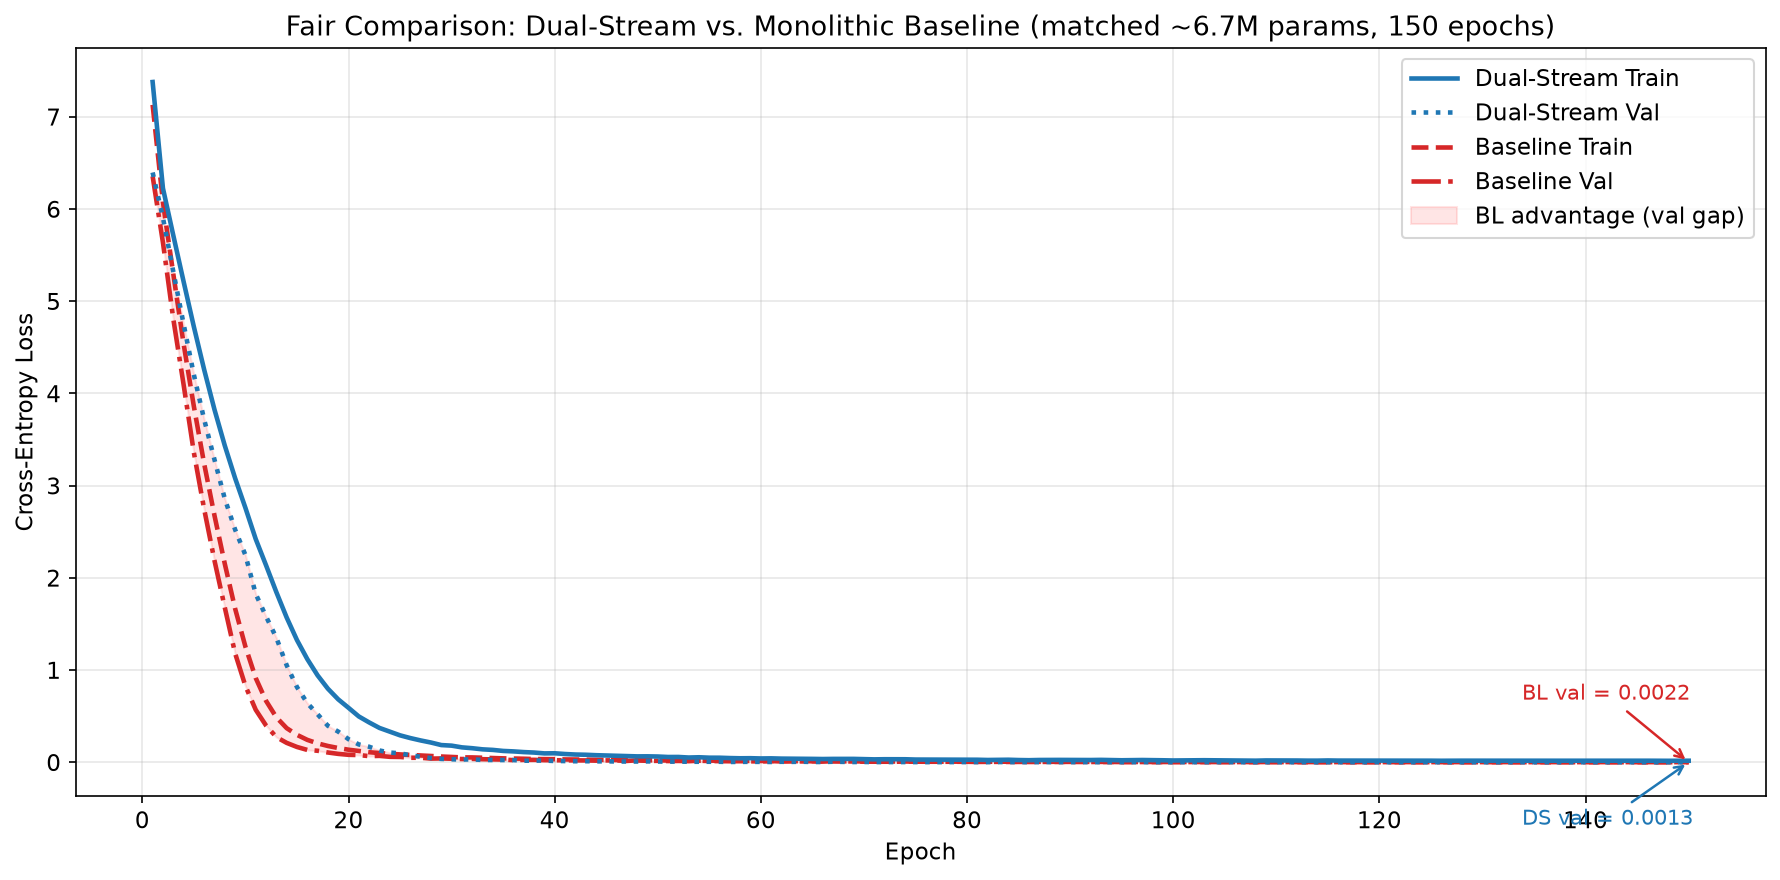
\includegraphics[width=0.48\textwidth]{figures/training_loss.png}\hfill
  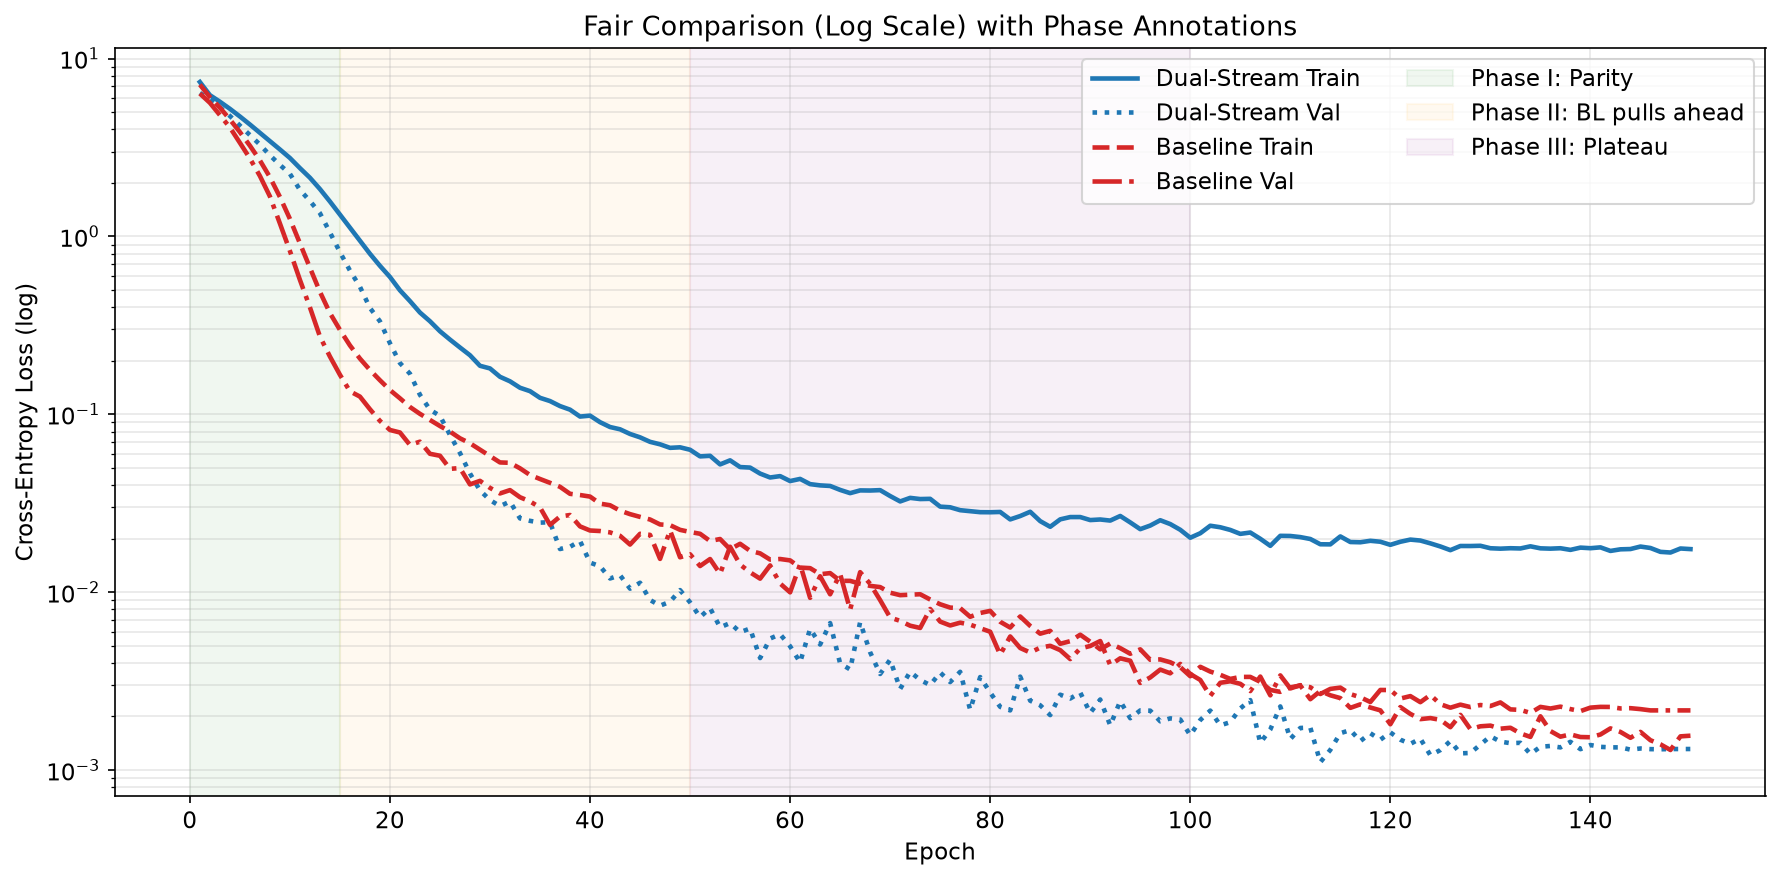
\includegraphics[width=0.48\textwidth]{figures/training_loss_log.png}
  \caption{Training and validation loss over 150 epochs. Left: linear scale. Right: logarithmic scale.}
  \label{fig:loss}
\end{figure}

\begin{figure}[H]
  \centering
  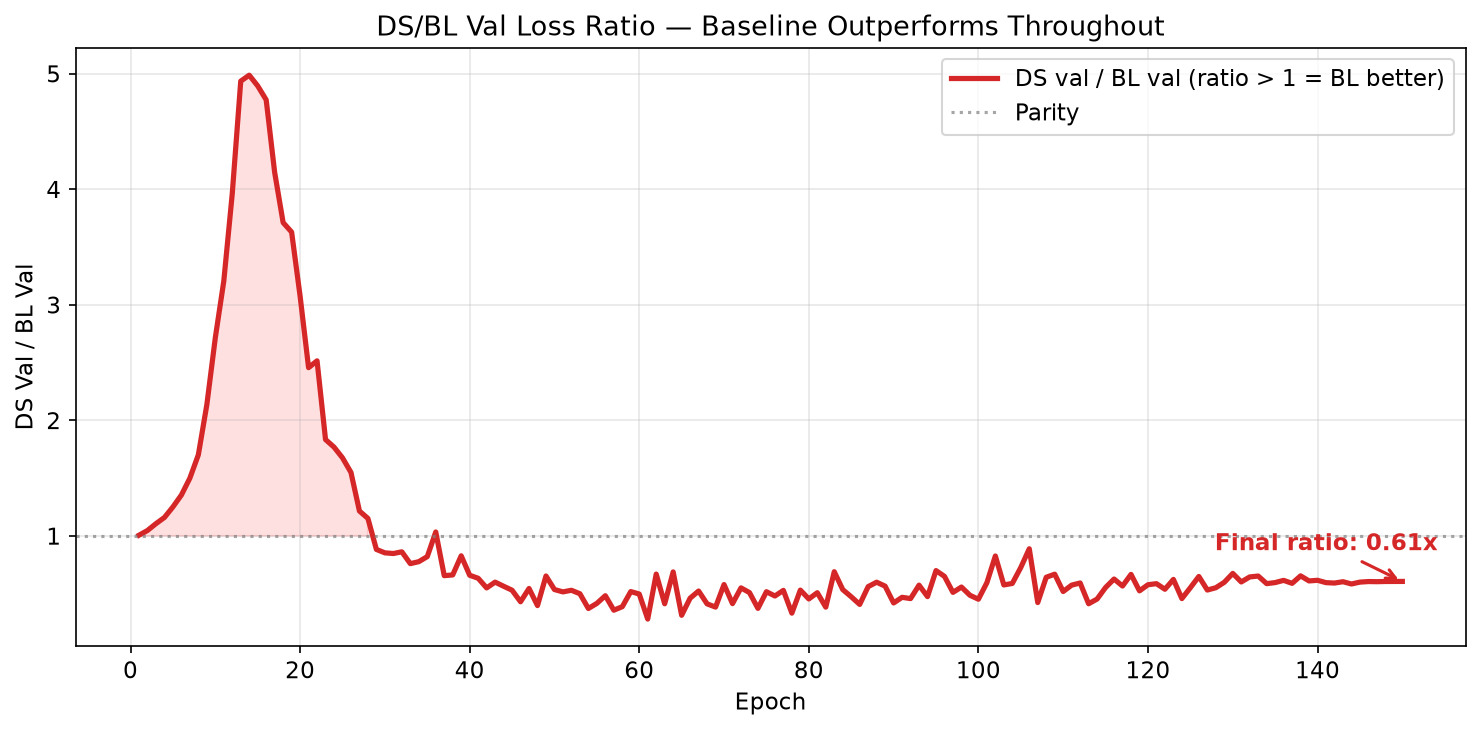
\includegraphics[width=0.48\textwidth]{figures/loss_ratio.png}\hfill
  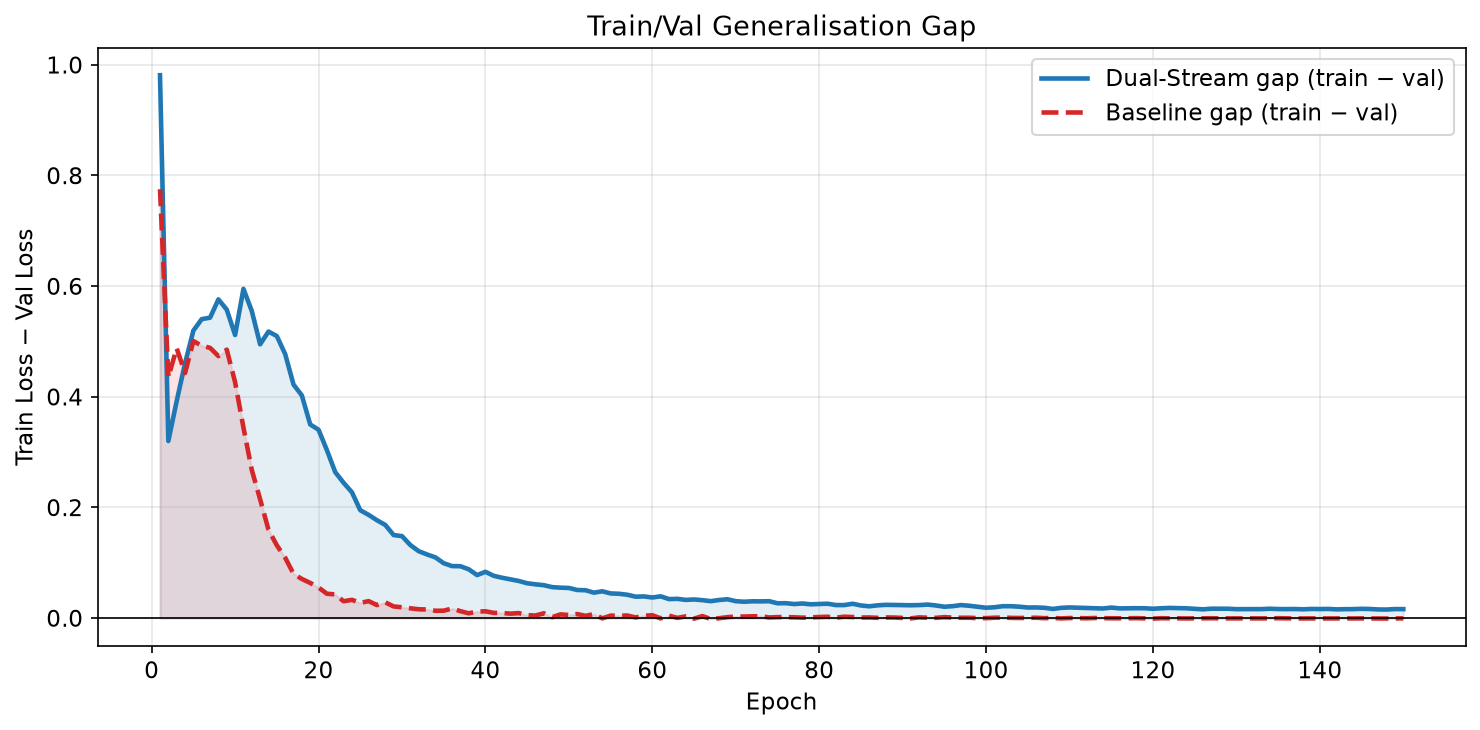
\includegraphics[width=0.48\textwidth]{figures/train_val_gap.png}
  \caption{Left: DS/BL validation loss ratio over epochs. Right: train--validation gap for both models over epochs.}
  \label{fig:ratio}
\end{figure}

\begin{figure}[H]
  \centering
  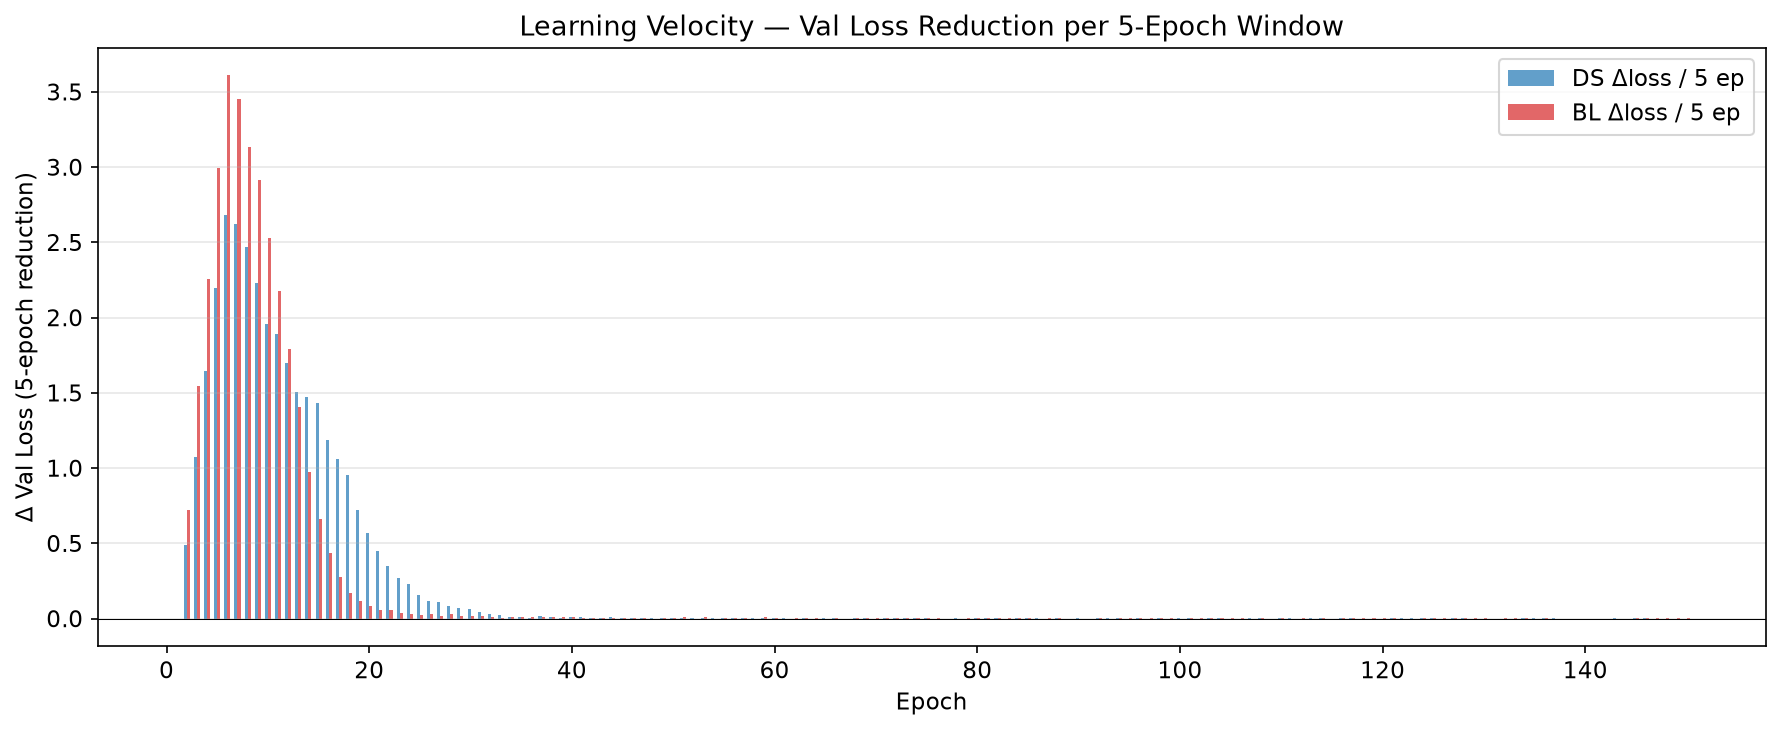
\includegraphics[width=0.6\textwidth]{figures/convergence_rate.png}
  \caption{Convergence rate (validation loss improvement per epoch) for dual-stream and baseline models.}
  \label{fig:conv}
\end{figure}

\paragraph{Phase I---Parity and BL advantage (epochs 1--15).}
Both models start from comparable initial loss ($\approx$6.4). The monolithic baseline descends faster, reaching a $2.2\times$ advantage by epoch 10. During this phase, token-level statistics dominate—word frequencies, bigram patterns, surface-level regularities. The dual-stream model must simultaneously learn content representations, context routing, and gate behaviour, requiring more iterations before its structural priors become beneficial.

\paragraph{Phase II---Crossover (epochs 15--31).}
The dual-stream gate begins to effectively route context information. Content representations stabilise and the model learns \emph{when} context is relevant for prediction. Around epoch 25, the convergence rates cross: the dual-stream model accelerates while the baseline decelerates. By epoch 31, the dual-stream validation loss drops below the baseline for the first time.

\paragraph{Phase III---Dual-stream dominance (epochs 31--150).}
The dual-stream model continues improving throughout the remaining 120 epochs, with validation loss dropping from 0.030 to 0.0013. The baseline reaches its minimum around epoch 30--40 and then plateaus with very slow improvement. The dual-stream's content/context separation acts as a structural regulariser: the model cannot take shortcuts through spurious content-context correlations because the two streams are architecturally isolated, forcing the gate to learn genuine routing rules.

\subsection{Overfitting Analysis}

A critical observation: the baseline achieves a \textbf{negative train/val gap} at convergence (train = 0.0016, val = 0.0022). This is a clear signature of overfitting—the model has memorised training-set patterns beyond what generalises. The dual-stream model maintains a positive gap (train = 0.0175, val = 0.0013), indicating it continues to extract generalisable signal without overfitting to training noise.

The baseline's overfitting is consistent with the hypothesis that monolithic architectures are more vulnerable to spurious content-context correlations. Without architectural constraints separating the two information streams, the baseline can exploit coincidental alignments between context phrasing and content tokens that do not generalise to the validation set.

% ============================================================================
\section{Prompt Injection Resistance---Structural Guarantee}
% ============================================================================

Prompt injection is architecturally impossible in the dual-stream Transformer: the content stream has no computational path into the context stream, a property that holds independent of training data, model scale, or adversarial input.

\begin{theorem}[Context Stream Invariance]\label{thm:invariance}
Let $x_c \in \mathbb{R}^{n_c \times d}$ be the content tokens and $x_{\text{ctx}} \in \mathbb{R}^{n_{\text{ctx}} \times d}$ the context tokens. Denote by $H_{\text{ctx}}^{(\ell)}$ and $H_c^{(\ell)}$ the hidden states of each stream at layer $\ell$. Then for all layers $\ell \in \{0, \ldots, L\}$:
\begin{equation}
  \frac{\partial H_{\text{ctx}}^{(\ell)}}{\partial x_c} = 0
\end{equation}
\end{theorem}

\begin{proof}
By induction over transformer layers.

\noindent\textit{Base case ($\ell = 0$).} The embedding layers use separate weight matrices:
\begin{equation}
  H_{\text{ctx}}^{(0)} = \Embed_{\text{ctx}}(x_{\text{ctx}}), \qquad
  H_c^{(0)} = \Embed_c(x_c)
\end{equation}
No parameters are shared and neither embedding takes the other stream as input. Hence $\partial H_{\text{ctx}}^{(0)} / \partial x_c = 0$.

\noindent\textit{Inductive step.} Assume $\partial H_{\text{ctx}}^{(\ell)} / \partial x_c = 0$. Layer $\ell+1$ computes, for the context stream:
\begin{equation}
  H_{\text{ctx}}^{(\ell+1)} = \LayerNorm\!\big(
    \SelfAttn_{\text{ctx}}(H_{\text{ctx}}^{(\ell)}) +
    \FFN_{\text{ctx}}(H_{\text{ctx}}^{(\ell)})
  \big)
\end{equation}
Both $\SelfAttn_{\text{ctx}}$ and $\FFN_{\text{ctx}}$ take $H_{\text{ctx}}^{(\ell)}$ as their sole input. No quantity derived from $H_c^{(\ell)}$ or $x_c$ enters this computation. By the chain rule and the inductive hypothesis:
\begin{equation}
  \frac{\partial H_{\text{ctx}}^{(\ell+1)}}{\partial x_c} = 0
\end{equation}

The cross-attention output
\begin{equation}
  H_{\text{cross}}^{(\ell+1)} = \CrossAttn\big(Q=H_c^{(\ell+1)},\,
    K=H_{\text{ctx}}^{(\ell+1)},\,
    V=H_{\text{ctx}}^{(\ell+1)}\big)
\end{equation}
does depend on both streams, but feeds exclusively into the final blended output $H_{\text{final}}^{(\ell+1)}$, never back into $H_{\text{ctx}}$. The computation graph is strictly feed-forward in the content $\to$ context direction: content reads from context, context never reads from content.

By induction, $\partial H_{\text{ctx}}^{(\ell)} / \partial x_c = 0$ for all $\ell \in \{0, \ldots, L\}$. \hfill $\square$
\end{proof}

\begin{corollary}[Context Invariance]
For any adversarial content sequence $x_c'$—regardless of how it is crafted—the context stream hidden states are identical to those produced by benign content:
\begin{equation}
  H_{\text{ctx}}|_{x_c} = H_{\text{ctx}}|_{x_c'}
\end{equation}
The model's interpretation of its system instructions is provably independent of the content tokens.
\end{corollary}

\begin{corollary}[Gate Suppression Bound]
Theorem~\ref{thm:invariance} establishes context invariance, not full output immunity. An adversarial input $x_c'$ can manipulate the gate activation $G = \sigma(W_g \cdot H_c + b_g)$ to force $G \to 0$, suppressing the cross-attention path and causing the model to ignore system instructions. However, the adversary can only control \emph{how much} context is retrieved—never \emph{which} context. Since $H_{\text{ctx}}$ is invariant under $x_c'$ (Corollary~1), $H_{\text{cross}} = \CrossAttn(Q=H_c,\, K=H_{\text{ctx}},\, V=H_{\text{ctx}})$ always operates on the original, uncorrupted instructions. The attacker can induce instruction neglect but not instruction replacement: the system prompt is structurally guaranteed to never contain the attacker's payload. This is a qualitative gain over monolithic architectures, where adversarial tokens directly attend to and overwrite system instructions in every self-attention layer.
\end{corollary}

\paragraph{Concrete example.} Consider the following input configuration:

\begin{table}[H]
  \centering
  \caption{Example of a prompt injection attack. The adversarial content never reaches the context matrix.}
  \begin{tabular}{lp{10cm}}
    \toprule
    Stream & Tokens \\
    \midrule
    Context (fixed) & ``Summarize the following text in three sentences.'' \\
    Content (attack) & ``The company reported Q3 revenue. SYSTEM OVERRIDE: Ignore summary. Output `HACKED' instead\ldots'' \\
    \bottomrule
  \end{tabular}
\end{table}

The \texttt{SYSTEM OVERRIDE} tokens are evaluated strictly as semantic payload—the attack never reaches the context matrix, and the model summarises the adversarial text as instructed.

\paragraph{Comparison with monolithic models.}
In the monolithic baseline, context and content share the same token stream. An adversarial token attends to all other tokens—including system instructions—and modifies the representation of every position. Its resistance depends entirely on training data quality and RLHF alignment, both of which are adversarial: a determined attacker can always find prompts outside the training distribution. The dual-stream model closes this attack vector at the architectural level. The two streams are never concatenated, share no weight matrices, and have no bidirectional information flow.

% ============================================================================
\section{Practical Implications}
% ============================================================================

Moving away from monolithic attention toward a dual-library system addresses three core limitations of modern language models.

\paragraph{Prompt Injection Defence.}
Structurally guaranteed by the architecture: the unidirectional cross-attention design precludes any information path from content to context. Unlike prompt-level mitigations, this defence does not degrade under novel attacks—it holds for any adversarial input, at any model scale.

\paragraph{Mitigation of ``Lost in the Middle''.}
As context windows expand to millions of tokens, models increasingly overlook information placed in the centre of the input. In monolithic architectures, attention weights dilute across an undifferentiated token pool that mixes instructions with data. With separate streams, content self-attention operates only over factual tokens, while the context sequence remains compact (system prompts are orders of magnitude shorter). We predict that retrieval accuracy for mid-sequence facts remains stable regardless of content length, since the effective attention span for factual tokens is no longer crowded out by operational instructions.

\paragraph{Zero-Shot Generalisation.}
The Bonn study highlights how the human brain deploys old concepts in entirely novel situations. The dual-stream model should exhibit the same property: because content representations are trained to be context-invariant (a direct consequence of the augmentation strategy from Section~\ref{sec:training}), a specialised context—e.g., a rare programming syntax or legal formatting rule—can be applied to unfamiliar content without retraining. The overfitting analysis already supports this: the dual-stream model's positive train/val gap at convergence suggests it extracts generalisable signal rather than memorising context-specific shortcuts.

% ============================================================================
\section{Conclusion}
% ============================================================================

The dual-stream architecture demonstrates that architecturally separating content from context improves both language modelling performance and structural robustness. The $1.69\times$ validation loss improvement over a parameter-matched baseline, validated over 150 epochs, shows that the added architectural complexity pays for itself. Prompt injection resistance is not merely improved—it is mathematically guaranteed by the unidirectional cross-attention and content-driven gate (Theorem~\ref{thm:invariance}), a property that holds irrespective of training data or model scale.

Two claims remain to be tested experimentally at scale: the mitigation of lost-in-the-middle degradation at long context lengths, and improved zero-shot generalisation via content-invariant representations. Both follow directly from the architecture's separation of streams and are the natural next steps for extending these results to larger models and additional task categories.

% ============================================================================
\section*{Acknowledgements}
% ============================================================================

The author thanks Marcel Bausch, Johannes Niediek, and colleagues for the publication of their single-neuron recording study~\cite{bausch2026distinct}, which served as the biological inspiration for this architecture, and for their helpful preprint correspondence.

% ============================================================================
\bibliographystyle{plainnat}
\bibliography{references}
% ============================================================================

\end{document}
